% Build with build.ps1: isolates stale auxiliary files, runs XeLaTeX twice.
\documentclass[12pt,a4paper]{article}
\usepackage{fontspec}
\usepackage{polyglossia}
\setdefaultlanguage{russian}
\setotherlanguage{english}
\setmainfont{Times New Roman}
\setmonofont{Consolas}
\usepackage{amsmath,amssymb}
\usepackage{graphicx,booktabs,float}
\usepackage{geometry,setspace}
\usepackage{xcolor,listings}
\usepackage[unicode,hidelinks]{hyperref}
\geometry{left=25mm,right=20mm,top=20mm,bottom=20mm}
\onehalfspacing
\setlength{\parindent}{1.25cm}
\setlength{\emergencystretch}{2em}
\graphicspath{{figures/}}
\lstset{language=Python,basicstyle=\ttfamily\small,breaklines=true,
  frame=single,rulecolor=\color{black!20},columns=fullflexible,
  keepspaces=true,showstringspaces=false,tabsize=4,
  keywordstyle=\color{blue!45!black},commentstyle=\color{black!55},
  aboveskip=0.6\baselineskip,belowskip=0.6\baselineskip}
% Generated by lab2.py; do not edit.
\newcommand{\NPoints}{97}
\newcommand{\TimeStep}{4}
\newcommand{\Duration}{384}
\newcommand{\SlopeFree}{196{,}86}
\newcommand{\InterceptFree}{1031{,}87}
\newcommand{\DiffusionFree}{49{,}21}
\newcommand{\RSquared}{0{,}9819}
\newcommand{\SlopeZero}{237{,}59}
\newcommand{\DiffusionZero}{59{,}40}
\newcommand{\RmseFree}{276{,}11}
\newcommand{\RmseZero}{548{,}08}
\newcommand{\MaxRelativeResidual}{29{,}3}


\begin{document}
\begin{titlepage}
\begin{center}
\begin{spacing}{1.3}
\textbf{МИНИСТЕРСТВО ОБРАЗОВАНИЯ РЕСПУБЛИКИ БЕЛАРУСЬ}\\[0.25cm]
\textbf{БЕЛОРУССКИЙ ГОСУДАРСТВЕННЫЙ УНИВЕРСИТЕТ}\\[0.25cm]
\textbf{ФАКУЛЬТЕТ МЕХАНИКО-МАТЕМАТИЧЕСКИЙ}\\[0.25cm]
\textbf{Кафедра веб-технологий и компьютерного моделирования}
\end{spacing}
\vspace{4.6cm}
\textbf{БРОУНОВСКОЕ ДВИЖЕНИЕ}\\[0.4cm]
Лабораторная работа
\end{center}
\vspace{3.6cm}
\noindent\hspace*{0.48\textwidth}\begin{minipage}{0.52\textwidth}
\begin{spacing}{1.0}
Панасика Владислава Александровича\\
обучающегося 4 курса специальности\\
«Математика и компьютерные науки»\\[0.6cm]
Научный руководитель:\\
ассистент КФОиПИ,\\
Полякова Яна Владимировна
\end{spacing}
\end{minipage}
\vfill
\begin{center}Минск, 2026\end{center}
\end{titlepage}
\setcounter{page}{2}

\tableofcontents
\newpage
\section{Цель работы и исходные данные}
Изучить броуновское движение и проверить зависимость среднего квадрата
смещения частицы от времени, предсказываемую формулой Эйнштейна.

Обработка выполнена по предоставленной таблице
\texttt{tablitsa\_pyltsa\_lr.xls}. На первом листе имеются
\NPoints{} полных пар координат $(x_i,y_i)$, измеренных через равные
промежутки времени $\tau=\TimeStep$ с. Последние три строки с номерами
98--100 не содержат координат и исключены из расчётов; остальные два листа
пусты. Таким образом, $n=\NPoints$, а продолжительность записи равна
$(n-1)\tau=\Duration$ с.

Координаты даны в пикселях. Масштаб изображения в мкм/пиксель, температура,
вязкость среды и радиус наблюдаемой частицы в таблице не указаны. Поэтому
результаты выражены в пиксель$^2$, а оценка коэффициента диффузии ---
в пиксель$^2$/с. Это позволяет исследовать зависимость от времени,
но не сравнить численно $D$ с формулой Стокса--Эйнштейна в единицах СИ.

По методичке установка включает микроскоп, цифровую камеру и компьютер;
наблюдается движение микрочастиц в эмульсии. В настоящей работе
использована уже полученная последовательность координат.

\section{Теоретические сведения}
Броуновское движение --- непрерывное хаотическое движение малых частиц,
взвешенных в жидкости или газе, под действием теплового движения молекул
среды. Удары молекул не компенсируются в каждый момент времени, поэтому
частица испытывает случайные изменения скорости и положения.

Уравнение Ланжевена для частицы массы $m$ имеет вид
\begin{equation}
 m\frac{d\mathbf v}{dt}=-\gamma\mathbf v+\mathbf F_{\mathrm c}(t),
 \qquad \langle\mathbf F_{\mathrm c}(t)\rangle=0,
 \qquad \gamma=\frac1b=6\pi\eta a,
\end{equation}
где $b$ --- подвижность, $\eta$ --- динамическая вязкость,
$a$ --- радиус сферической частицы. Сила Стокса направлена против скорости
частицы относительно жидкости. Закон Стокса применим при малом числе
Рейнольдса; влияние близких стенок в этой модели не учитывается.

Коэффициент диффузии задаётся соотношением Стокса--Эйнштейна:
\begin{equation}
 D=bk_{\mathrm B}T=\frac{k_{\mathrm B}T}{6\pi\eta a},
 \label{eq:diffusion}
\end{equation}
где $k_{\mathrm B}$ --- постоянная Больцмана, $T$ --- абсолютная температура.
При $t\gg\tau_v=mb=m/\gamma$ средний квадрат смещения вдоль одной оси
равен $2Dt$. Для наблюдаемой двумерной проекции
\begin{equation}
 \boxed{\langle\Delta s^2(t)\rangle
 =\langle\Delta x^2(t)\rangle+\langle\Delta y^2(t)\rangle=4Dt.}
 \label{eq:einstein}
\end{equation}
В трёхмерном пространстве $\langle\Delta r^2\rangle=6Dt$.
Коэффициент 4 в данной работе определяется двумя наблюдаемыми координатами.

Формула~\eqref{eq:einstein} относится к среднему \emph{квадрату} смещения.
Среднеквадратичное смещение есть корень из этой величины:
$s_{\mathrm{rms}}=\sqrt{\langle\Delta s^2\rangle}=\sqrt{4Dt}$;
оно растёт как $\sqrt t$.

\section{Метод обработки}
Для девяти лагов $k=1,\ldots,9$ взяты интервалы
$t_k=k\tau=4,8,\ldots,36$ с. Для каждого лага использованы все
перекрывающиеся пары $(i,i+k)$:
\begin{align}
 \Delta s_{i,k}^{\,2}&=(x_{i+k}-x_i)^2+(y_{i+k}-y_i)^2,\\
 M_k\equiv\widehat{\langle\Delta s^2\rangle}(t_k)
 &=\frac{1}{n-k}\sum_{i=1}^{n-k}\Delta s_{i,k}^{\,2}.
 \label{eq:estimate}
\end{align}
При $k=1$ имеется 96 пар, при $k=9$ --- 88 пар. Всего рассчитано
828 квадратов смещений. Усреднение по времени одной достаточно длинной
траектории используется как оценка среднего по ансамблю при предположении
стационарных, эргодических приращений.

Например, для первых двух положений $(520,441)$ и $(559,446)$:
\[
 \Delta s_{1,1}^{\,2}=(559-520)^2+(446-441)^2=1546\ \text{пиксель}^2.
\]
При $k=1$ сумма по всем 96 парам равна $128956$ пиксель$^2$, откуда
$M_1=128956/96=1343{,}29$ пиксель$^2$.

Для проверки формы зависимости использованы две невзвешенные
аппроксимации методом наименьших квадратов:
\begin{enumerate}
 \item $M(t)=at+c$ --- для оценки линейности и свободного сдвига;
 \item $M(t)=At$ --- модель формулы Эйнштейна с $M(0)=0$.
\end{enumerate}
Вторая оценка имеет явный вид
\begin{equation}
 A=\frac{\sum_k t_k M_k}{\sum_k t_k^2},\qquad D_0=\frac A4.
\end{equation}
Для свободной прямой $D_{\mathrm{св}}=a/4$, а качество аппроксимации
описано центрированным коэффициентом
\begin{equation}
 R^2=1-\frac{\sum_k[M_k-(at_k+c)]^2}
 {\sum_k(M_k-\overline M)^2}.
\end{equation}
Для каждой модели также вычислено
$\mathrm{RMSE}=\sqrt{\frac19\sum_k(M_k-M_{\mathrm{модель}}(t_k))^2}$.
Эти показатели характеризуют отклонения девяти точек от прямых,
но не являются погрешностью $D$.

\section{Результаты расчётов}
\begin{table}[H]
\centering
\caption{Средние квадраты смещений по всем доступным парам}
\label{tab:msd}
\begin{tabular}{rrrrr}
\toprule
$k$ & $t_k$, с & $n-k$ & $\sum_i\Delta s_{i,k}^{\,2}$, пиксель$^2$
& $M_k$, пиксель$^2$\\
\midrule
\input results/msd_rows.tex
\bottomrule
\end{tabular}
\end{table}

\begin{figure}[H]
\centering
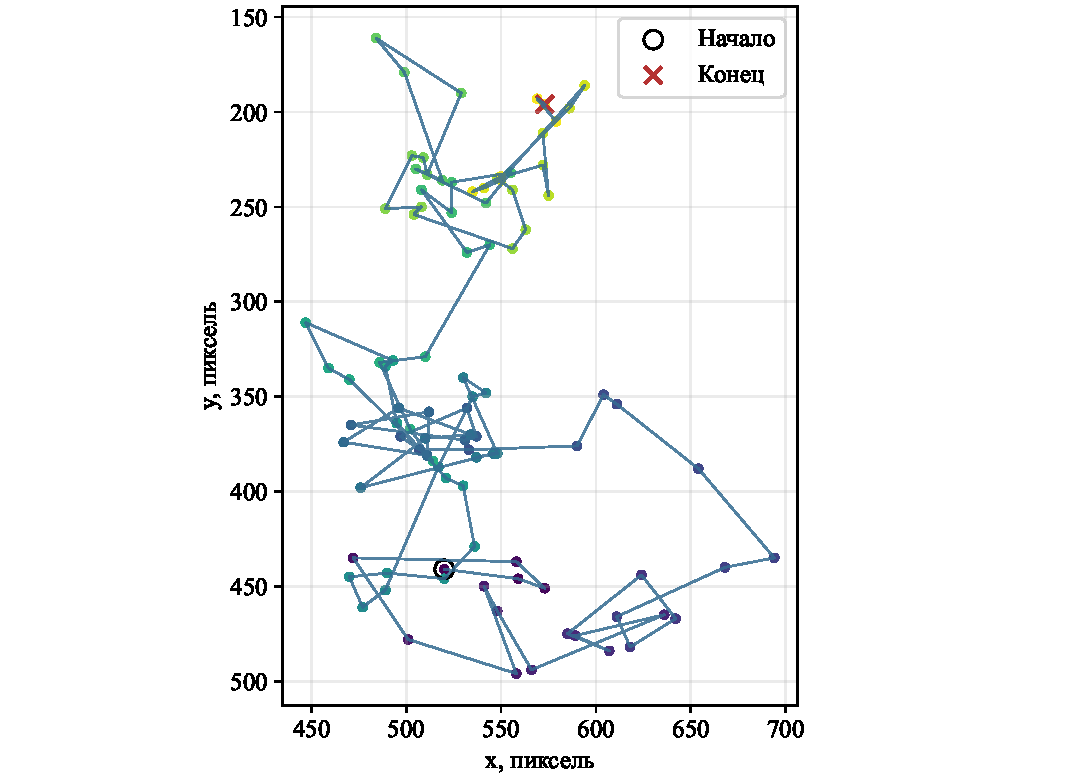
\includegraphics[width=0.75\textwidth]{trajectory.pdf}
\caption{Траектория по 97 положениям. Ось $y$ направлена вниз,
как в экранной системе координат; это не влияет на квадраты смещений.}
\end{figure}

\begin{figure}[p]
\centering
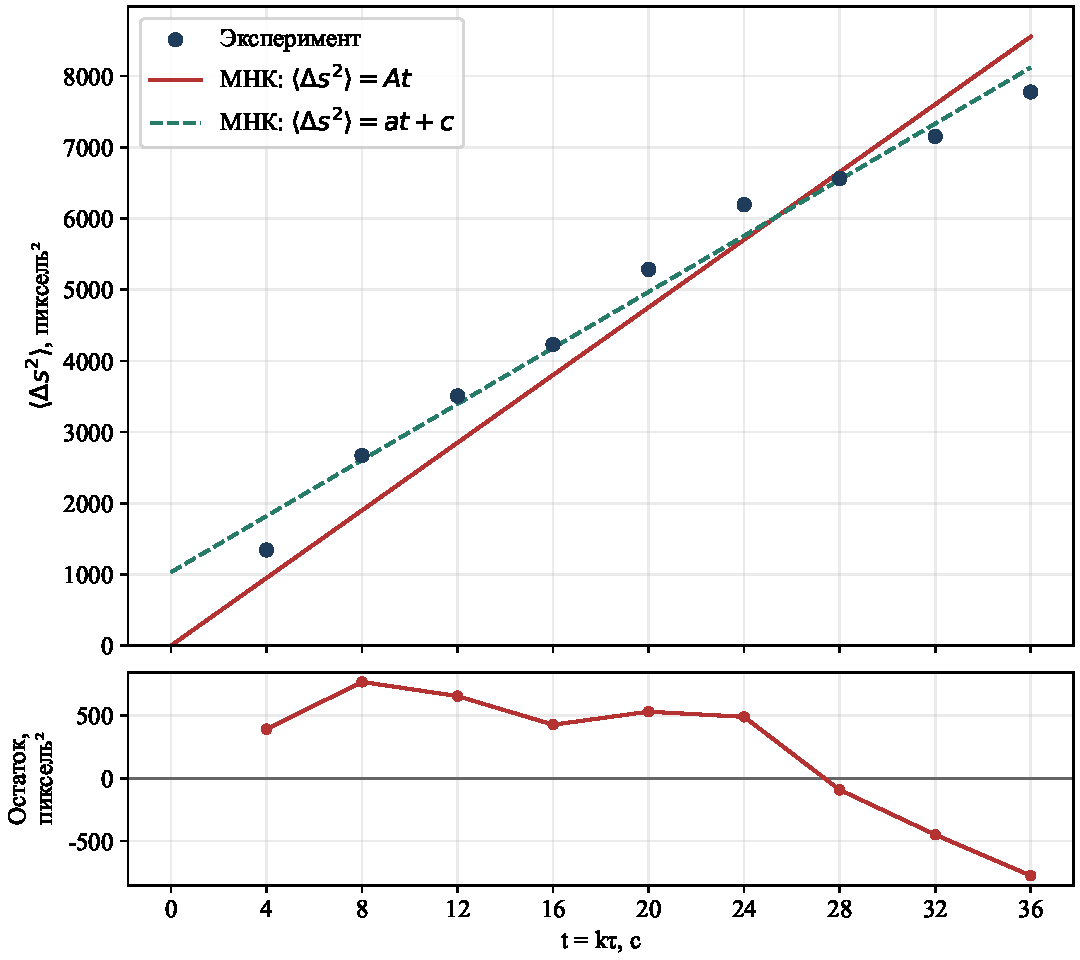
\includegraphics[width=0.95\textwidth]{msd.pdf}
\caption{Средний квадрат смещения и две аппроксимации.
Внизу показаны остатки $M_k-At_k$ для прямой через начало координат.}
\label{fig:msd}
\end{figure}

Свободная линейная аппроксимация даёт
\begin{equation}
 M(t)=\SlopeFree\,t+\InterceptFree,
 \qquad R^2=\RSquared,
\end{equation}
где $t$ выражено в секундах, $M$ --- в пиксель$^2$.
Здесь $a=\SlopeFree$ пиксель$^2$/с,
$c=\InterceptFree$ пиксель$^2$,
$D_{\mathrm{св}}=\DiffusionFree$ пиксель$^2$/с,
а $\mathrm{RMSE}_{\mathrm{св}}=\RmseFree$ пиксель$^2$.

При обязательном прохождении прямой через начало координат:
\begin{equation}
 M(t)=\SlopeZero\,t,\qquad
 \boxed{D_0=\DiffusionZero\ \text{пиксель}^2/\text{с}},
\end{equation}
а $\mathrm{RMSE}_0=\RmseZero$ пиксель$^2$.
Максимальное относительное отклонение экспериментальной точки от этой
модели, $\max_k|M_k-At_k|/M_k$, составляет
\MaxRelativeResidual\,\%.

\subsection{Обсуждение и ограничения}
Рост $M_k$ близок к линейному на интервалах 4--36 с.
Вместе с тем положительный сдвиг свободной прямой и структура остатков
показывают заметное отклонение от строгой пропорциональности $M=4Dt$.
Следовательно, большое $R^2$ само по себе не доказывает прохождения
зависимости через начало координат.

Две оценки $D$ зависят от выбора модели: приблизительно
$49{,}2$ и $59{,}4$ пиксель$^2$/с. Последнее число является оценкой
в рамках принудительно выбранной модели~\eqref{eq:einstein},
а не независимо подтверждённой константой среды.

Перекрывающиеся смещения и средние для разных лагов статистически
зависимы. Поэтому стандартные ошибки обычной регрессии по девяти точкам
нельзя считать надёжной экспериментальной погрешностью коэффициента
диффузии. Доверительный интервал в настоящей обработке не определяется.

На результат могут влиять конечная длина записи, ошибки определения
координат, размытие при экспозиции, потоки жидкости и близость стенок.
По одной траектории нельзя однозначно установить причину отклонений.
Даже направленное смещение начала и конца записи само по себе не доказывает
наличия постоянного потока. Поправка на дрейф здесь не вводилась.

Если впоследствии будет известен масштаб $q$ в мкм/пиксель, то
\[
 M_{\text{мкм}^2}=q^2M_{\text{пиксель}^2},\qquad
 D_{\text{мкм}^2/\text{с}}=q^2D_{\text{пиксель}^2/\text{с}}.
\]
Для перехода к м$^2$/с последнее значение нужно умножить на $10^{-12}$.

\clearpage
\section{Программная реализация}
Расчёты выполнены в \texttt{lab2.py} с помощью NumPy, чтение Excel ---
с помощью xlrd, графики построены Matplotlib. Скрипт сохраняет исходные
координаты, все пары смещений, сводную таблицу, параметры аппроксимаций
и рисунки. Числа и строки таблицы подключаются к отчёту из автоматически
создаваемых файлов \texttt{results/values.tex} и
\texttt{results/msd\_rows.tex}.

Основной фрагмент вычисления средних квадратов смещений:
\begin{lstlisting}
for lag in range(1, MAX_LAG + 1):
    delta = xy[lag:] - xy[:-lag]
    squared = np.sum(delta**2, axis=1)
    summary.append((lag, lag * tau, len(squared),
                    squared.sum(), squared.mean()))
\end{lstlisting}
Здесь \texttt{xy} имеет размер $97\times2$, а число строк
\texttt{delta} равно $n-k$. Ни начальное положение для всех пар,
ни длина ломаной траектории вместо смещения не используются.

Фрагмент двух аппроксимаций:
\begin{lstlisting}
slope, intercept = np.linalg.lstsq(
    np.column_stack((t, np.ones_like(t))),
    msd, rcond=None
)[0]
slope_zero = np.dot(t, msd) / np.dot(t, t)
D_free = slope / 4
D_zero = slope_zero / 4
\end{lstlisting}
Порядок повторного запуска и сборки приведён в \texttt{README.md}.

\section{Ответы на контрольные вопросы}
\subsection*{1. Что называется броуновским движением?}
Непрерывное хаотическое движение малых частиц, взвешенных в жидкости
или газе, вызванное некомпенсированными ударами молекул окружающей среды.
Оно служит наблюдаемым проявлением теплового движения молекул.

\subsection*{2. Какие частицы можно назвать броуновскими?}
Это частицы, существенно крупнее молекул среды, для которых тепловые
флуктуации вызывают заметное случайное перемещение. Примеры --- мелкие
капли жира в эмульсии, частицы дыма и мелкие взвеси.
В методичке рассматриваются капли диаметром примерно $0{,}2$--$1$ мкм.
Эти размеры характеризуют описанную установку и не определяют универсальных
границ броуновского движения; радиус частицы из предоставленной таблицы
по ним не устанавливается.

\subsection*{3. Почему силу действия молекул жидкости разделяют на
случайную силу и силу вязкого трения?}
Взаимодействие со средой имеет среднюю и флуктуационную составляющие.
Средняя сила при движении частицы относительно жидкости направлена
против скорости и при малой скорости равна $-\gamma\mathbf v$.
Отклонение мгновенной силы от её среднего описывается случайной силой
с нулевым средним. Трение рассеивает энергию упорядоченного движения,
а случайная сила поддерживает тепловые флуктуации. В равновесии их
интенсивности связаны соотношением флуктуации--диссипации.

\subsection*{4. Зависит ли сила вязкого трения шарообразной частицы
от её диаметра?}
Да. При применимости закона Стокса
\[
 \mathbf F_{\mathrm{тр}}=-6\pi\eta a\mathbf v
 =-3\pi\eta d\mathbf v,\qquad d=2a.
\]
При одинаковых вязкости среды и относительной скорости модуль силы
прямо пропорционален диаметру. При этом из~\eqref{eq:diffusion}
следует $D\propto1/d$: более крупная частица диффундирует медленнее.

\section{Вывод}
По 97 положениям частицы вычислены средние квадраты смещений
для девяти интервалов времени от 4 до 36 с. Эксперимент показывает
приближённо линейный рост среднего квадрата смещения с временем
($R^2=\RSquared$ для свободной прямой), согласующийся с диффузионным
характером движения.

Строгое выполнение зависимости $\langle\Delta s^2\rangle=4Dt$
по имеющимся данным не установлено: свободный член отличен от нуля,
а отклонения от прямой через начало достигают \MaxRelativeResidual\,\%.
В рамках модели через начало координат получено
$D_0\approx\DiffusionZero$ пиксель$^2$/с;
при свободном сдвиге --- $D_{\mathrm{св}}\approx\DiffusionFree$
пиксель$^2$/с. Перевод в физические единицы требует калибровки изображения.

\end{document}
